\documentclass{article}
\usepackage{graphicx} % Required for inserting images

\title{Homework Exercise 3}
\author{Angelica Ortiz 11191225, Daniel Nägele 11180610}
\date{May 2026}

\begin{document}

\maketitle
\thispagestyle{empty}
\newpage

\tableofcontents
\newpage

\section{Exercise 3 -- RFID}

The RFID system is based on Dynamic Frame ALOHA and contains $N=4$ tags.

The collision resolution efficiency is defined as:

\[
\eta = \frac{N}{E[T]} = \frac{4}{E[T]}
\]

The expected resolution time for each initial frame size $r_1$ is:

\[
E[T] = r_1 + \sum_{i=0}^{3} P(S=i)L_{4-i}
\]

where $S$ is the number of successfully transmitted tags in the first frame.

Using the given values:

\[
L_2 = 4, \qquad L_3 = \frac{51}{8}=6.375
\]

and computing $L_4$ for $r=N=4$:

\[
L_4 =
\frac{4 + 0.1875L_3 + 0.5625L_2}{1-0.15625}
\]

\[
L_4 =
\frac{4 + 0.1875\cdot 6.375 + 0.5625\cdot 4}{0.84375}
= 8.8241
\]

The resulting efficiencies are:

\[
\begin{array}{c|c|c}
r_1 & E[T] & \eta \\
\hline
1 & 9.8241 & 0.4072 \\
2 & 9.5995 & 0.4167 \\
3 & 8.9544 & 0.4467 \\
4 & 8.8241 & 0.4533 \\
5 & 9.0377 & 0.4426 \\
6 & 9.4661 & 0.4226 \\
\end{array}
\]

The maximum efficiency is obtained for:

\[
r_1 = 4
\]

with:

\[
\eta_{\max} \approx 0.4533
\]

This result is expected because the optimal initial frame size is equal to the number of tags, $r_1=N=4$. In this case, the probability of having one tag per slot is maximized, reducing both collisions and empty slots.

\begin{figure}[h]
    \centering
    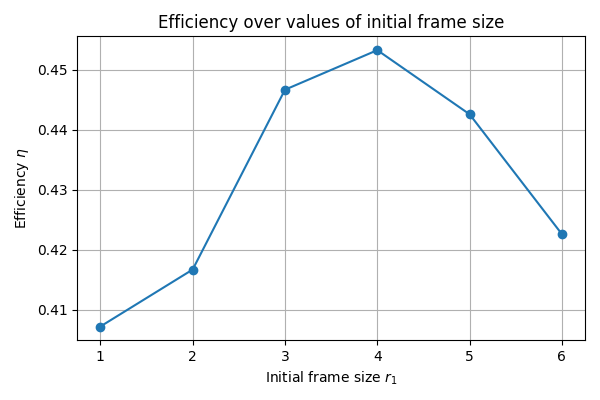
\includegraphics[width=0.8\textwidth]{plot.png}
    \caption{Efficiency over values of initial frame size}
    \label{fig:efficiency}
\end{figure}

\end{document}